\documentclass[3p]{elsarticle}
\usepackage{ae,aecompl}
\usepackage[T1]{fontenc}
\usepackage[utf8]{inputenc}
\usepackage{pgfplots}
\usepackage{pst-plot}
\usepackage{tikz}
\usepgfplotslibrary{external}
\tikzexternalize
\usepackage{amsmath}
\usepackage{amssymb}
\usepackage{gensymb}
\usepackage{upgreek}
\usepackage{float}
\usepackage{indentfirst}
\parskip=0pt

\begin{document}

\begin{frontmatter}

\title{The effect of electric field on potentiometric Scanning Electrochemical Microscopic images}
\cortext[cor]{Corresponding author}
\author[akiss]{András Kiss\corref{cor}}
\address[akiss, gnagy]{Department of General and Physical Chemistry, Faculty of Sciences, University of Pécs, 7624 Pécs, Ifjúság útja 6, Hungary}
%\address[akiss, gnagy]{János Szentágothai Research Centre, University of Pécs, 7624 Pécs, Ifjúság Útja 20, Hungary}
\ead{akiss@gamma.ttk.pte.hu}
\author[dfilotas]{Dániel Filotás}
\ead{filotasdaniel@gmail.com}
\author[gnagy]{Géza Nagy}
\ead{g-nagy@gamma.ttk.pte.hu}


\begin{abstract}

Scanning Electrochemical Microscopy (SECM) is an invaluable tool in corrosion science.
It allows the selective imaging of a particular ionic species being released at the anodic sites, using ion-selective microelectrodes (ISMEs) as scanning probes.
An often studied phenomenon is galvanic corrosion, which involves two metals in electrical contact, immersed in the same electrolyte.
The measured potential of the ISME is thought to depend only on the activity of primary ion.
However, an electric field is also formed as a result of the potential difference between the surfaces of the galvanic pair, 
which has a direct influence on the potential of the microelectrode; the measured potential is the sum of these two.
The potential difference caused by the electric field can be substantially large, exceeding that of the potential difference associated with the activity of the primary ion.
In this paper, we present experimental evidence of this, and investigate the extent to which it influences the final image. 
\end{abstract}
\begin{keyword}
	scanning electrochemical microscopy \sep potentiometry \sep galvanic corrosion \sep electric field
\end{keyword}
\end{frontmatter}

\section{Introduction}

In the past decade, potentiometric SECM - or in other words used by the experts of this field Scanning Ion Selective Electrode Technique (SIET) - has become very popular among corrosion scientists\cite{lamaka, ZnISME, diamondel, cutedge, H+selective, simulating}. The most broad spread application is the visualization of galvanic corrosion\cite{amperopot, chloride, spatiozn, fezn}.
Galvanic corrosion occurs when two dissimilar metals are connected both electrically and immersed in the same electrolyte. The electric coupling results the preferential and accelerated dissolution of the anode, while reduces corrosion rate of the cathode. The spatial separation of the anodic and the cathodic sites makes the complex corrosion processes easily interpretable and due to the increased corrosion rate conveniently short exposure times are sufficient to obtain convincing concentration distributions in the solution adjacent to the corroding sample.

Despite these beneficial circumstances, quantitative evaluation of galvanic corrosion using potentiometric SECM often fails due to – up to now – unrevealed reasons.
Izquierdo et. al. reported discrepant results comparing vertical approaching curves towards the cathode of the Mg-Fe galvanic couple obtained by amperometric $O_2$ detection and potentiometric pH measurements \cite{pH15}. Local alkalinization could be detected even at 2 mm tip-substrate distance, whereas oxygen concentration reached the bulk level at ca. 900 $\upmu$m height. The phenomenon was explained by the contribution of the electric field to the potentiometric signal.  
In another works, $Mg^{2+}$ above Mg alloy disc galvanically coupled to iron detected with Mg ISME highly exceeded the upper limit of detection of the probe \cite{overmg1, overmg2, overmg3}.
On the other hand, pMg values fallen behind lower limit of detection of Mg ISMEs scanning above cathodically polarized magnesium strips \cite{belowmg}. 

These phenomenon could be explained by a contribution of the electric field to the measured potential. The potential difference between the surfaces of the anode and the cathode causes an electric field to be formed. The potential difference between the points where the electrodes are located is added to the potential difference associated with the primary ion activity at the tip of the measuring electrode:

\begin{equation}
\Delta E=E_M-E_R + (\phi_M - \phi_R)
\label{eq:potential}
\end{equation}

where $\Delta E$ is the measured potential difference, $E_R$ is the potential of the reference electrode, $\phi_M$ and $\phi_R$ are the potentials in the electric field at the measuring and reference electrodes, respectively. $E_M$ is the potential of the measuring electrode:

\begin{equation}
E_M = S \times lg[Mg^{2+}] + E_M^o
\label{eq:measuring}
\end{equation}

where $S$ is the slope of the calibration curve of the potentiometric cell with respect to the primary ion, and $E_M^o$ is the standard potential.

\begin{figure}
\centering
% trim = top left bottom right
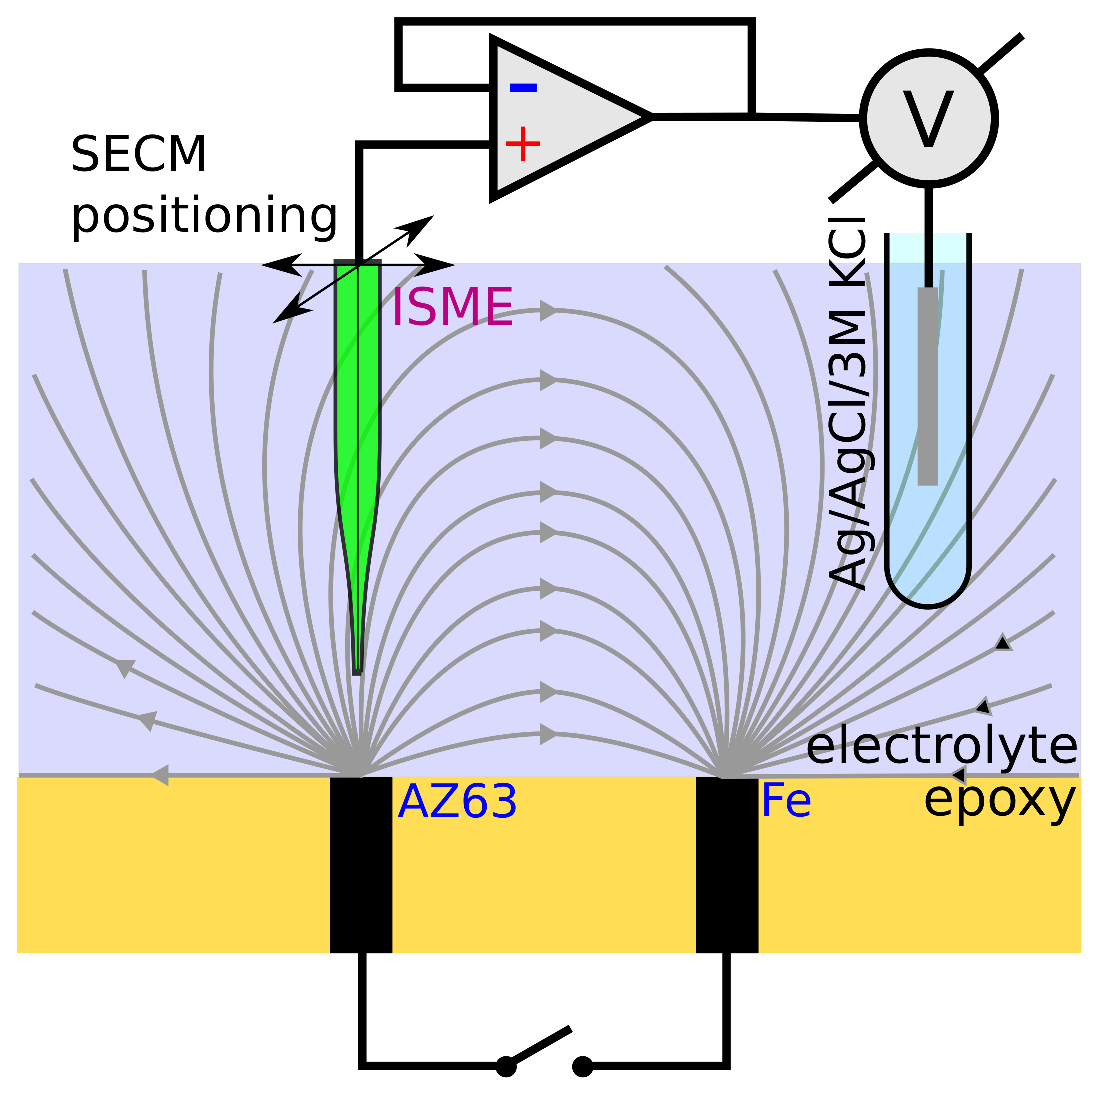
\includegraphics[width=0.5\textwidth]{abstract.eps}
\caption{Caption.}
\label{fig:abstract}
\end{figure}

The effect of the electric field on the measured potential difference has been investigated in this paper. The galvanic corrosion of the AZ63 Mg-Al alloy and iron was used as a model system.


\section{Material and methods}


The preparation of solid contanct $Mg^{2+}$ selective microelectrodes was adopted from a previous work \cite{overmg3}. Micropipettes were pulled from borosilicate capillaries (outer diameter $\oslash$ = 1.5 mm, inner dia. $\oslash$ = 1.0 mm, obtained from Hilgenberg GmbH, Malsfeld, Germany) with a Sutter Instruments P-30 type vertical capillary puller (Novato, CA, USA). The micropipette were soaked in 1:1 $H_2SO_4$:$H_2O_2$ solution and washed with double deionized water. The capillaries were silanized by 1 hour exposition the saturated vapour of dichloro-dimethyl-silane in closed Petri dishes at 120 $\celsius$. A poly-ethylen-dioxy-thiophene (PEDOT) coated carbon fiber of 33 $\upmu$m diameter (obtained as a generous gift from Specialty Materials, Lowell, MA, USA) served as the solid contact of the ISME. The PEDOT was electrochemically polymerized to the carbon fiber in 0.1 M EDOT-containing $BMIM-PF_6$ ionic liquid solution. 10 consecutive cyclic voltammetry cycles were taken in -0.9 $\leq$ E $\leq$ 1.3 V range. The doping step was performed in 0.1 M KCl aqueous solution by applying 15 consecutive potential cycles in the -0.9 $\leq$ E $\leq$ 0.8 V range. The membrane components were purchased from Fluka (Buchs, Switzerland). The cocktail contains N,N''-Octamethylene-bis(N'-heptyl-N'-methyl-methylmalonamide inophore, 2-nitrophenyl-octyl ether emollient, PVC, potassium-[tetrakis-4-chlorophenyl]-borate and tetrahydrofuran. Eventually, the micropipette wre frontfilled with the coctail and the PEDOT coated carbon fiber was inserted in the lumen of the capillary.
The Mg ISMEs were calibrated by measuring their potential against Ag/AgCl/KCl (3M) reference electrode in tenfold diluted $MgCl_2$ solutions between $10^{-7}$ and $10^{-1}$ M concentrations. The activities were calculated using the Debye-Hückel theory. Nernstian relationship was found in between $10^{-1}$ and $10^{-5}$ M, the equation of the linear portion of the calibration curve is -29.5mV/decade+98.3mV ($R^2=0.9997$). The lower limit of detection was pMg=5.3. 

The (Mg/Al)/Fe galvanic couple target was prepared from  AZ63 Mg/Al alloy and high purity Fe wires with identical diameter of 0.76 mm. The wires were mounted in an epoxy resin sleeve (Struers, Ballerup, Denmark)., exposing only the disk shaped surfaces and allowing to make electric contact at the rear of the mould. Frontal surface of the mould was first polished with SiC paper down to 4000 grit, then with 1.0, 0.3 $\upmu$m alumina powder.

SECM experiments were carried out employing homemade instrument operated with custom software. The sample was placed at the bottom of the electrochemical cell, whereas the local potential values of the Mg ISMEs were measured with against a Ag/AgCl (3M KCl) reference electrode. All the measurements were performed using a high input impedance eDAQ pH ISE isoPod USB(eDAQ Pty Ltd, Australia).

\section{Results and discussion}

First, consecutive approaching curves were recorded above the corroding AZ63 sample, while the galvanic connection with the iron sample was...

The moment the galvanic connection was established, there was an immediate rise of about 140 mV in the measured potential of the microelectrode [fig], which cannot possibly be attributed to the increase of $Mg^{2+}$ activity that far from the source. Also, a 140 mV rise would mean an increase of about 3.5 orders of magnitude in $Mg^{2+}$ activity in less then a second. Even if one argues it's possible 100 $\upmu$m from the source, it cannot be the case 1000 $\upmu$m from it. The only plausable explanation is that sudden change is due to the electric field formed between the two metals. 

\begin{figure}
\centering
\begin{tikzpicture}
\begin{axis}[ymin=-0.08, ymax=0.08, xmin=0, xmax=1000, xlabel={height, $\upmu$m}, ylabel={E vs. Ag/AgCl/3 M KCl, V}, clip marker paths=true, width=7cm, height=7cm, legend style={draw=none}, legend cell align=left]
\addplot [domain=0:1000, color=red] table {1.txt};
\addplot [domain=0:1000, color=red] table {2.txt};
\addplot [domain=0:1000, color=red] table {3.txt};
\addplot [domain=0:1000, color=red] table {4.txt};
\addplot [domain=0:1000, color=red] table {5.txt};
\addplot [domain=0:1000, color=red] table {6.txt};
\addplot [domain=0:1000, color=red] table {7.txt};
\addplot [domain=0:1000, color=blue] table {8.txt};
\addplot [domain=0:1000, color=blue] table {9.txt};
\addplot [domain=0:1000, color=blue] table {10.txt};
\addplot [domain=0:1000, color=blue] table {11.txt};
\addplot [domain=0:1000, color=blue] table {12.txt};
\addplot [domain=0:1000, color=blue] table {13.txt};
\addplot [domain=0:1000, color=green] table {14.txt};
\addplot [domain=0:1000, color=green] table {15.txt};
\node[anchor=north east] at (rel axis cs:0.98,0.98) {A};

%\node[black, above left] at (axis cs:0,-290) {pH 4};
%\node[black, above right] at (axis cs:0,-290) {pH 6};
%\addplot +[mark=none] coordinates {(0, -300)-.- (0, -100)};
%\draw [dashed, black] (axis cs:0,-300) -- (axis cs:0,-100);
%\addlegendentry{raw recording}
%\addlegendentry{$E = - 280 + 97 e^{-t/3.76}$}
%\addlegendentry{$E = - 280 + 97 (e^{-t/9} + e^{-t/0.5577})/2$}
\end{axis}
\end{tikzpicture}
\begin{tikzpicture}
\begin{axis}[ymin=-75, ymax=200, xmin=0, xmax=680, xlabel={time, s}, ylabel={E vs. Ag/AgCl/3 M KCl, mV}, clip marker paths=true, width=7cm, height=7cm, legend style={draw=none}, legend cell align=left]
\addplot [domain=-30:100, color=red, mark=*] table {on_off_100.txt};
\addplot [domain=-30:100, color=blue, mark=*] table {on_off_1000.txt};
\node[anchor=north east] at (rel axis cs:0.98,0.98) {B};

%\node[black, above left] at (axis cs:0,-290) {pH 4};
%\node[black, above right] at (axis cs:0,-290) {pH 6};
%\addplot +[mark=none] coordinates {(0, -300)-.- (0, -100)};
%\draw [dashed, black] (axis cs:0,-300) -- (axis cs:0,-100);
%\addlegendentry{raw recording}
%\addlegendentry{$E = - 280 + 97 e^{-t/3.76}$}
%\addlegendentry{$E = - 280 + 97 (e^{-t/9} + e^{-t/0.5577})/2$}
\end{axis}
\end{tikzpicture}

\caption[Transient response of the antimony microelectrode to analyte activity step.]{Transient response of the antimony microelectrode to analyte activity step.
The measuring and reference electrodes were dipped into buffer solutions with pH = 4 before the measurements started, and pH = 6 at t = 0 s, respectively.
Eq. \ref{eq:rc} was fitted (red line) on the measurement (gray marks) from the pH step to the end of the curve when potential reaches equilibrium in the pH = 6 buffer.}
\label{fig:transient}
\end{figure}





\def\s{0.35}
\begin{figure}
\centering
% trim = top left bottom right
\includegraphics[trim = 10mm 20mm 0mm 10mm, clip, width=\s\textwidth, angle=-90]{17012501.eps}\includegraphics[trim = 10mm 20mm 0mm 10mm, clip, width=\s\textwidth, angle=-90]{17012503_deconvoluted.eps}
\caption{Caption.}
\label{fig:label1}
\end{figure}





\section{Conclusions}
\section*{Acknowledgements}
This research was supported by the European Union and the State of Hungary, co-financed by the European Social Fund in the framework of T\'{A}MOP-4.2.4.A/ 2-11/1-2012-0001 'National Excellence Program' and T\'{A}MOP-4.2.2.A-11/1/KONV-2012-0065.

\section*{References}

\begin{thebibliography}{5}

\bibitem{lamaka}S.V. Lamaka, M.G. Taryba, M.L. Zheludkevich, M.G.S. Ferreira, Novel Solid-Contact Ion-Selective Microelectrodes for Localized Potentiometric Measurements Electroanalysis 21 (2009) 2447-2453.
\bibitem{ZnISME}J. Izquierdo, L. Nagy, Á.s Varga, I. Bitter, G. Nagy, R. M. Souto Scanning electrochemical microscopy for the investigation of corrosion processes: Measurement of  $Zn^{2+}$ spatial distribution with ion selective microelectrodes Electrochimica Acta 59 (2012) 398–403. 
\bibitem{diamondel}E.L. Silva, A.C. Bastos, M.A. Neto, R.F. Silva, M.G.S. Ferreira, M.L. Zheludkevich, F.J. Oliveira Novel diamond microelectrode for pH sensing Electrochemistry Communications 40 (2014) 31–34.
\bibitem{cutedge}A. Alvarez-Pampliega, S.V. Lamaka, M.G. Taryba, M. Madani, J. De Strycker, E. Tourwé, M.G.S. Ferreira, H. Terryn Cut-edge corrosion study on painted aluminum rich metallic coated steel by scanning vibrating electrode and micro-potentiometric techniques Electrochimica Acta 61 (2012) 107–117.	
\bibitem{H+selective}E. A. Zdrachek. A. G. Karotkaya, V. A. Nazarov,K. A. Andronchyk, L. S. Stanishevskii, V. V. Egorov, M. G. Taryba, D. Snihirova, M. Kopylovich, S. V. Lamaka $H^{+}$-selective microelectrodes with optimized measuring range for corrosion studies  Sensors and Actuators B 207 (2015) 967–975.
\bibitem{simulating}H. Shi, Z. Tian, T. Hu, F. Liu, E. H. Han, M. Taryba, S.V. Lamaka Simulating corrosion of Al2CuMg phase by measuring ionic currents, chloride concentration and pH Corrosion Science 88 (2014) 178–186.
\bibitem{amperopot}J. Izquierdo, L. Nagy, J. J. Santana, G. Nagy, R. M. Souto A novel microelectrochemical strategy for the study of corrosion inhibitors employing the scanning vibrating electrode technique and dual potentiometric/amperometric operation in scanning electrochemical microscopy: Application to the study of the cathodic inhibition by benzotriazole of the galvanic corrosion of copper coupled to iron Electrochimica Acta 58 (2011) 707–716.
\bibitem{chloride}V. A. Nazarov, M. G. Taryba, E. A. Zdrachek, K. A. Andronchyk, V. V. Egorov, S. V. Lamaka Sodium- and chloride-selective microelectrodes optimized for corrosion studies Journal of Electroanalytical Chemistry 706 (2013) 13–24.
\bibitem{spatiozn}E. Tada, S. Satoh, H. Kaneko,The spatial distribution of $Zn^{2+}$ during galvanic corrosion of a Zn/steel couple Electrochimica Acta 49 (2004) 2279–2285.
\bibitem{fezn}A.G. Marques M. Taryba A.S. Pan˜ao S. Lamaka A.M. Simoes Application of scanning electrode techniques for the evaluation of iron–zinc corrosion in nearly neutral chloride solutions Corrosion Science 104 (2016) 123-131.
\bibitem{pH15}J. Izquierdo, L. Nagy, I. Bitter, Ricardo M. Souto, G. Nagy 
Potentiometric scanning electrochemical microscopy for the local characterization of the electrochemical behaviour of magnesium-based materials Electrochimica Acta 87 (2013) 283–293.
\bibitem{overmg1}R. M. Souto, A. Kiss, J. Izquierd, L. Nagy, I. Bitter, G. Nagy Spatially-resolved imaging of concentration distributions on corroding magnesium-based materials exposed to aqueous environments by SECM Electrochemistry Communications 26 (2013) 25–28.
\bibitem{overmg2}R.M. Souto, J Izquierdo, J.J. Santana, A Kiss, L Nagy, G Nagy 
Progress in Scanning Electrochemical Micro scopy by Coupling Potentiometric and Amperometric Measurement Modes
In: Gabor Nagy, Gyula Pinczes, Gabor Pinter, Istvan Pocsi, Jozsef Prokisch, Gaspar Banfalvi
A Méndez-Vilas (szerk.)
Current microscopy contributions to advances in science and technology. Spain: Formatex Research Center, 2012. pp. 1407-1415.
\bibitem{overmg3}J. Izquierdo, A. Kiss, J. J. Santana, L. Nagy, I. Bitter, H. S. Isaacs, G. Nagy, R. M. Souto
Development of $Mg^{2+}$ Ion-Selective Microelectrodes for Potentiometric Scanning Electrochemical Microscopy Monitoring of Galvanic Corrosion Processes
Journal of the Electrochemical Society  160 (2013) 451-459. 
\bibitem{belowmg}J. Izquierdo, B. M. Fernández-Pérez, D. Filotás, Z. Őri, A. Kiss, R.T. Martín-Gómez, L. Nagy, G. Nagy, R. M. Souto Imaging of Concentration Distributions and Hydrogen Evolution on Corroding Magnesium Exposed to Aqueous Environments Using Scanning Electrochemical Microscopy Electroanalysis 28 (2016) 1–14.

\end{thebibliography}

\end{document}
